\section{Project Managment}
When managing a team, it is very important to know the skills of the individual team members properly.
This makes it possible to correctly use the skills of the individual team members and to distribute the right tasks to the right people. In our team we are made up of people who are familiar with hardware and IOT, as well as others who are more familiar with software or graphic design. At the beginning of the project the skills of the individual people were evaluated on a scale of 0 - 1 in order to find out who is best suited for which task.

\begin{figure}[H]
	\centering
	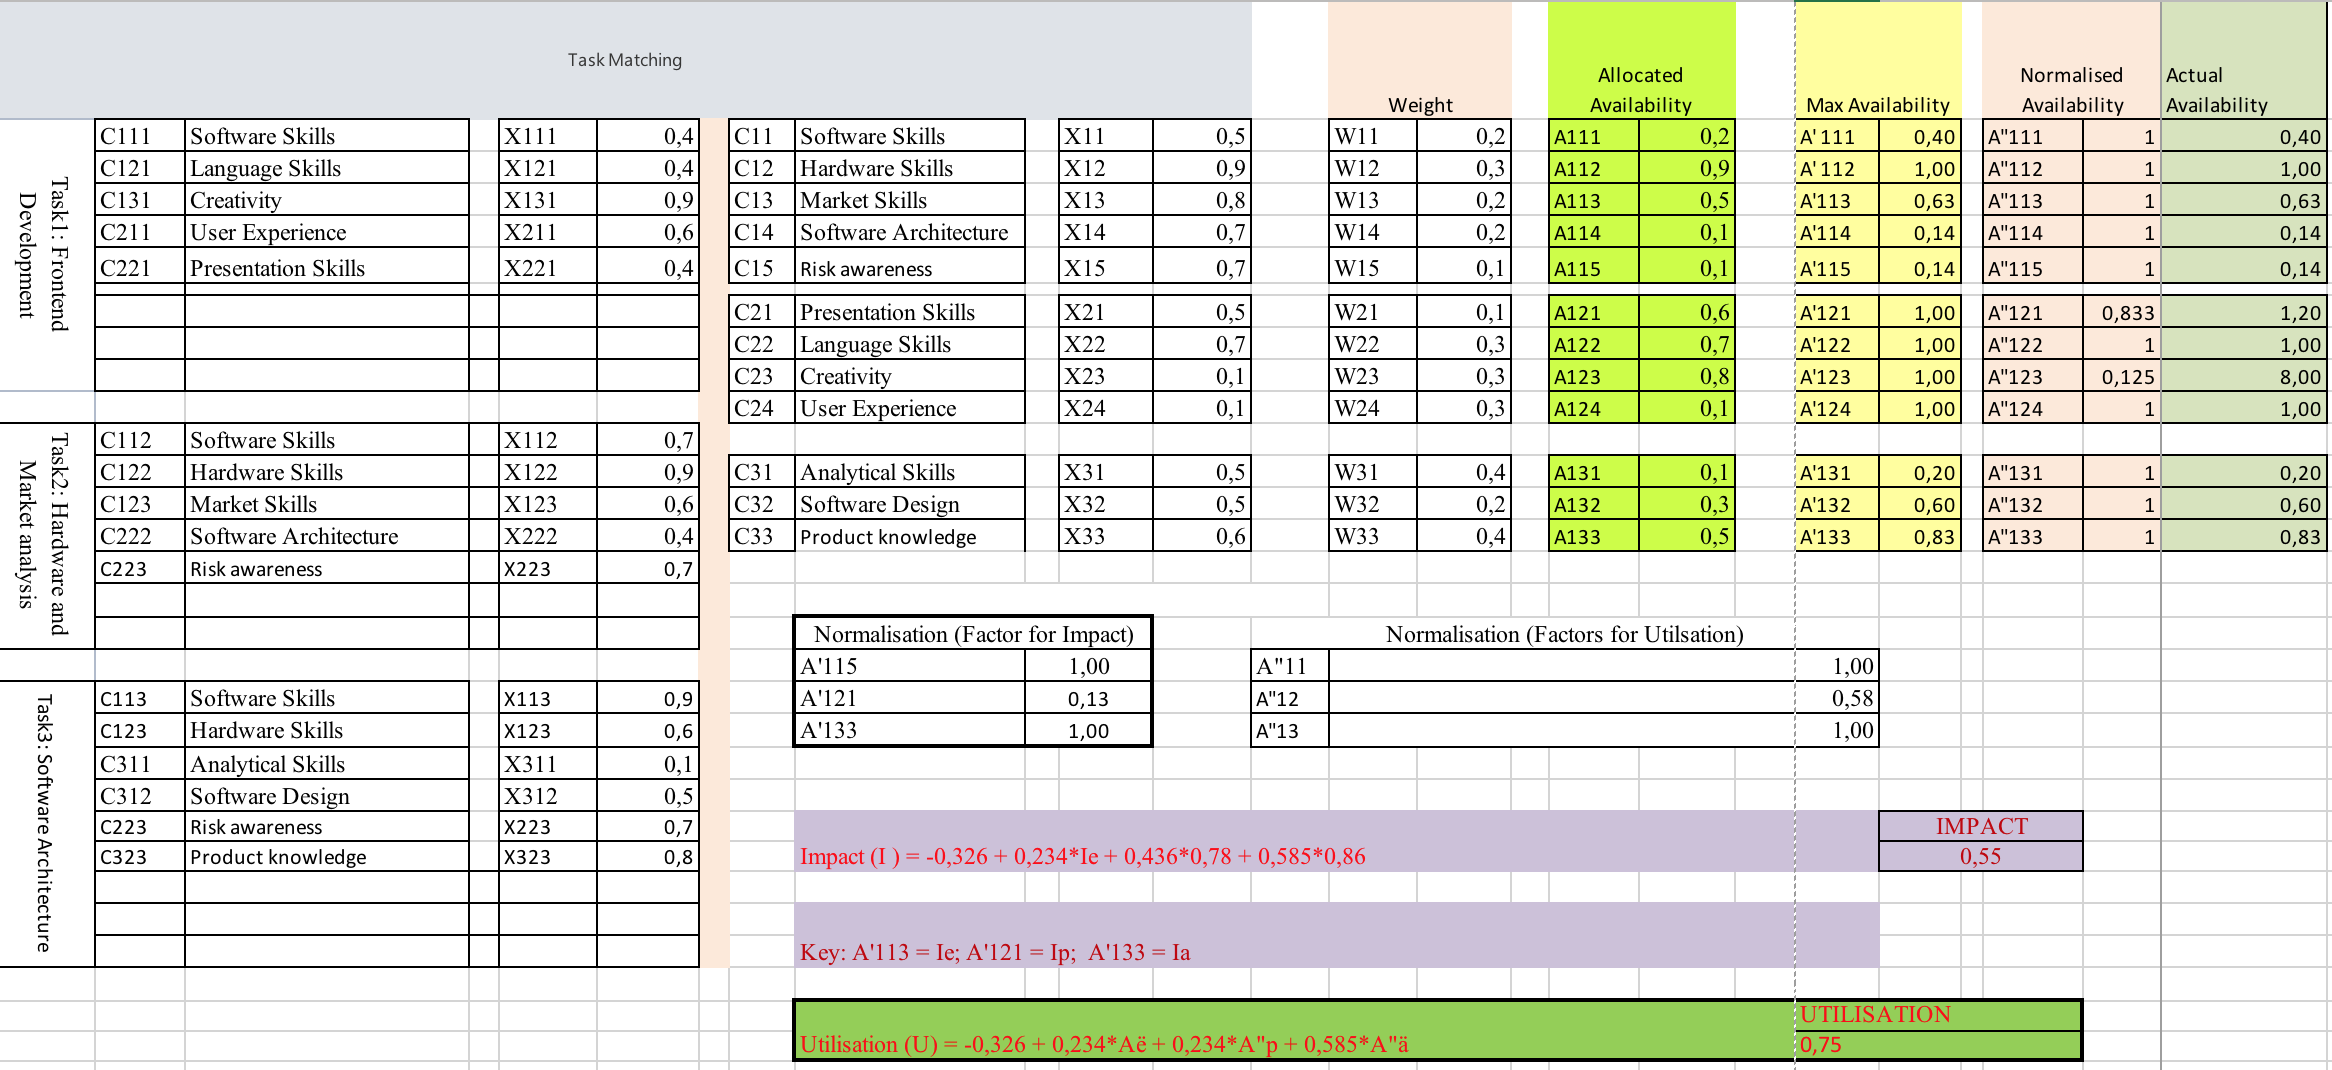
\includegraphics[width =1.05\textwidth]{images/evalTony.png}
	\caption{Evaluation Antonio Parrotta}
\end{figure}

\begin{figure}[H]
	\centering
	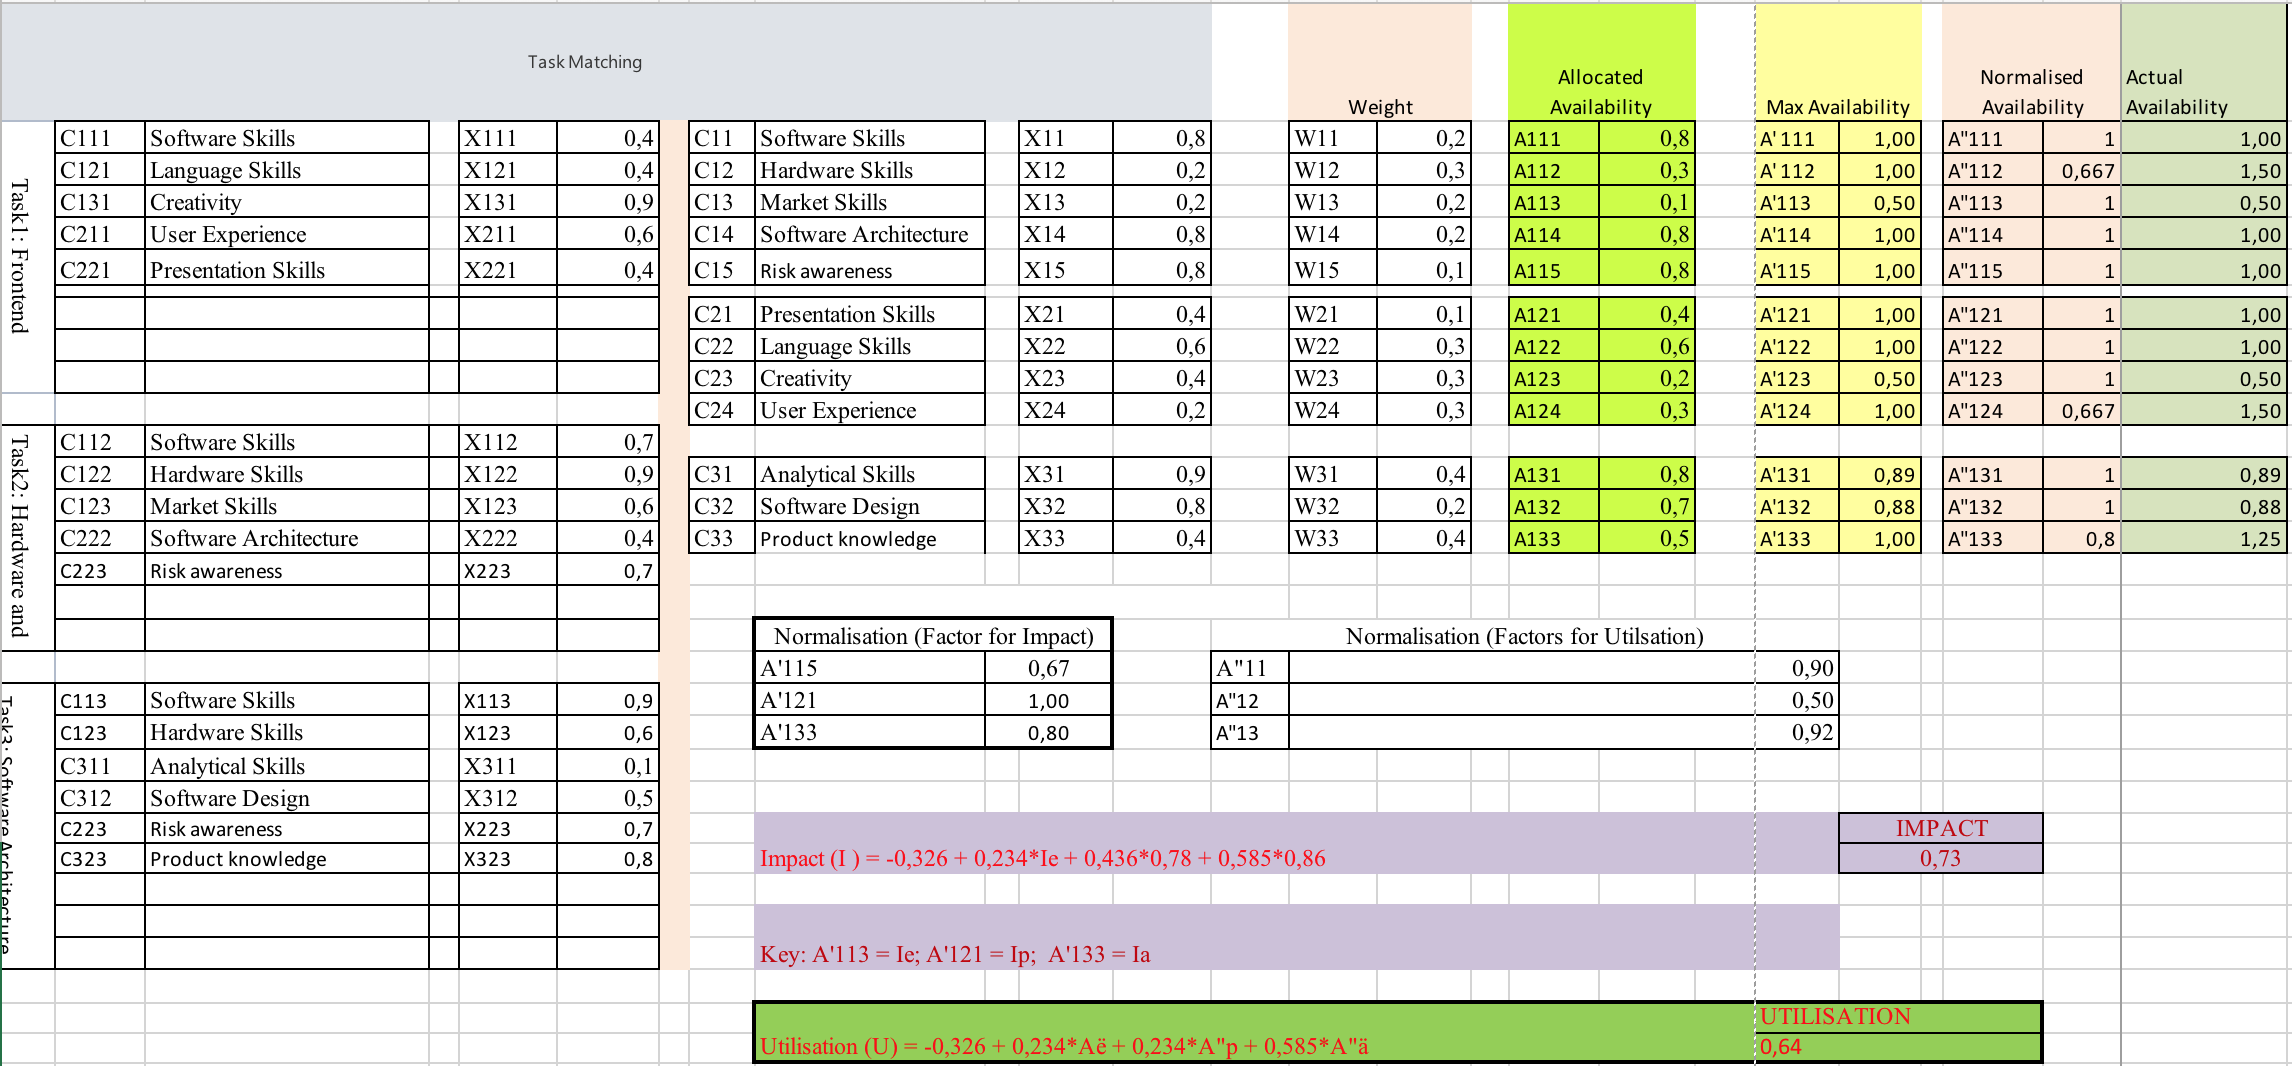
\includegraphics[width =1.05\textwidth]{images/evalChris.png}
	\caption{Evaluation Christoph Gschrey}
\end{figure}

\begin{figure}[H]
	\centering
	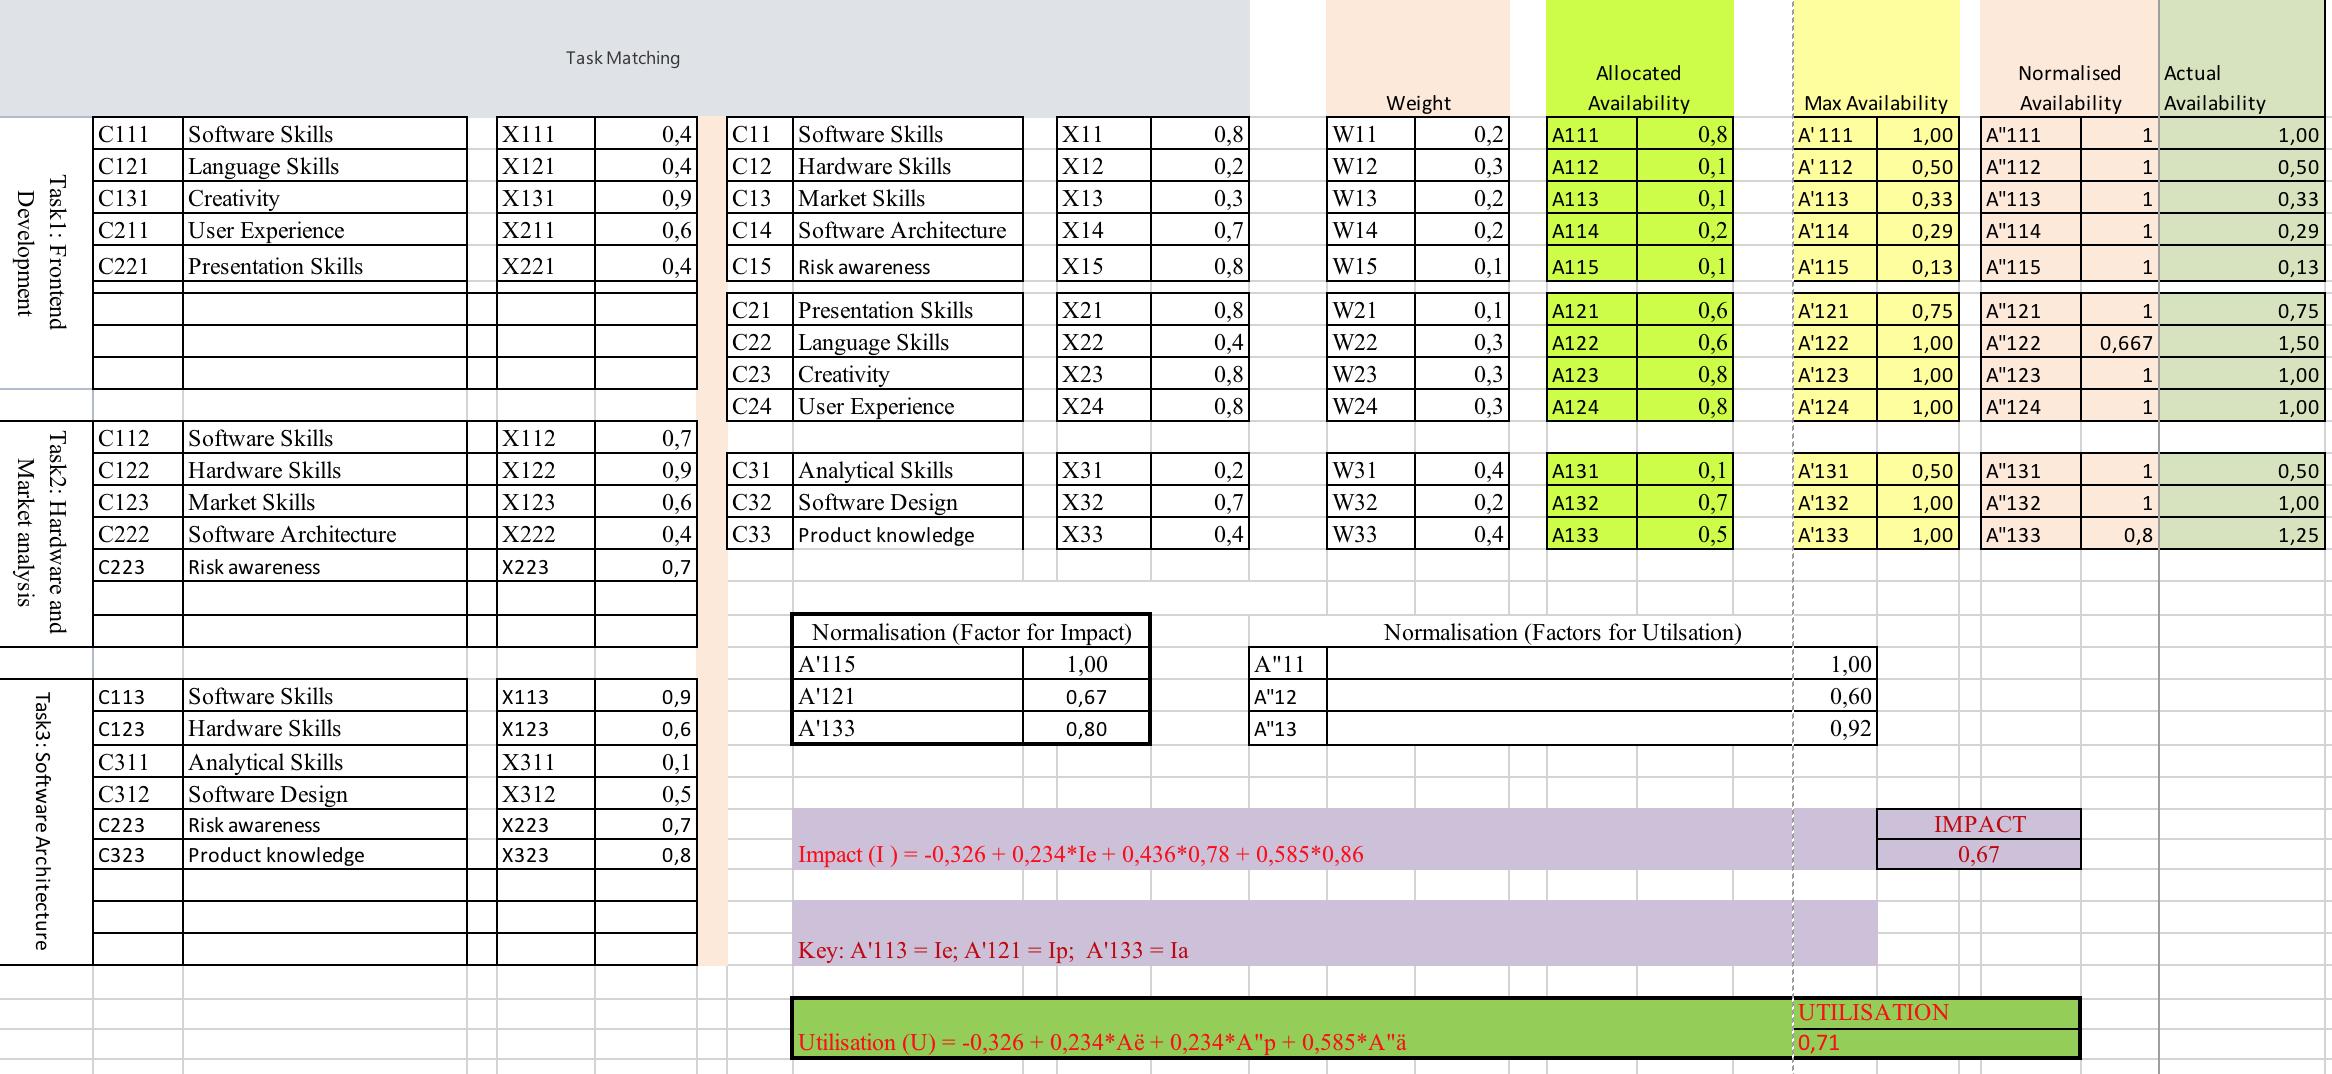
\includegraphics[width =1.05\textwidth]{images/evalDennis.png}
	\caption{Evaluation Dennis Mueller}
\end{figure}

